\documentclass[11pt]{article}

\newcommand{\yourname}{Zerun Tian}
\newcommand{\yourcollaborators}{}

\def\comments{0}
\setlength{\parindent}{0 in}
\setlength{\parskip}{0.1in}

\usepackage{graphicx}
\graphicspath{ {./} }

%format and packages

%\usepackage{algorithm, algorithmic}
\usepackage[noend]{algpseudocode}
\usepackage{amsmath, amssymb, amsthm}
\usepackage{enumerate}
\usepackage{enumitem}
\usepackage{framed}
\usepackage{verbatim}
\usepackage[margin=1.0in]{geometry}
\usepackage{microtype}
\usepackage{kpfonts}
\usepackage{palatino}
	\DeclareMathAlphabet{\mathtt}{OT1}{cmtt}{m}{n}
	\SetMathAlphabet{\mathtt}{bold}{OT1}{cmtt}{bx}{n}
	\DeclareMathAlphabet{\mathsf}{OT1}{cmss}{m}{n}
	\SetMathAlphabet{\mathsf}{bold}{OT1}{cmss}{bx}{n}
	\renewcommand*\ttdefault{cmtt}
	\renewcommand*\sfdefault{cmss}
	\renewcommand{\baselinestretch}{1.06}
\usepackage[usenames,dvipsnames]{xcolor}
\definecolor{DarkGreen}{rgb}{0.15,0.5,0.15}
\definecolor{DarkRed}{rgb}{0.6,0.2,0.2}
\definecolor{DarkBlue}{rgb}{0.2,0.2,0.6}
\definecolor{DarkPurple}{rgb}{0.4,0.2,0.4}
\usepackage[pdftex]{hyperref}
\hypersetup{
	linktocpage=true,
	colorlinks=true,				% false: boxed links; true: colored links
	linkcolor=DarkBlue,		% color of internal links
	citecolor=DarkBlue,	% color of links to bibliography
	urlcolor=DarkBlue,		% color of external links
}

%enclosure macros
\newcommand{\paren}[1]{\ensuremath{\left( {#1} \right)}}
\newcommand{\bracket}[1]{\ensuremath{\left\{ {#1} \right\}}}
\renewcommand{\sb}[1]{\ensuremath{\left[ {#1} \right\]}}
\newcommand{\ab}[1]{\ensuremath{\left\langle {#1} \right\rangle}}

%probability macros
\newcommand{\ex}[2]{{\ifx&#1& \mathbb{E} \else \underset{#1}{\mathbb{E}} \fi \left[#2\right]}}
\newcommand{\pr}[2]{{\ifx&#1& \mathbb{P} \else \underset{#1}{\mathbb{P}} \fi \left[#2\right]}}
\newcommand{\var}[2]{{\ifx&#1& \mathrm{Var} \else \underset{#1}{\mathrm{Var}} \fi \left[#2\right]}}

%useful CS macros
\newcommand{\poly}{\mathrm{poly}}
\newcommand{\polylog}{\mathrm{polylog}}
\newcommand{\zo}{\{0,1\}}
\newcommand{\pmo}{\{\pm1\}}
\newcommand{\getsr}{\gets_{\mbox{\tiny R}}}
\newcommand{\card}[1]{\left| #1 \right|}
\newcommand{\set}[1]{\left\{#1\right\}}
\newcommand{\negl}{\mathrm{negl}}
\newcommand{\eps}{\varepsilon}
\DeclareMathOperator*{\argmin}{arg\,min}
\DeclareMathOperator*{\argmax}{arg\,max}
\newcommand{\eqand}{\qquad \textrm{and} \qquad}
\newcommand{\ind}[1]{\mathbb{I}\{#1\}}
\newcommand{\sslash}{\ensuremath{\mathbin{/\mkern-3mu/}}}

%mathbb
\newcommand{\N}{\mathbb{N}}
\newcommand{\R}{\mathbb{R}}
\newcommand{\Z}{\mathbb{Z}}
%mathcal
\newcommand{\cA}{\mathcal{A}}
\newcommand{\cB}{\mathcal{B}}
\newcommand{\cC}{\mathcal{C}}
\newcommand{\cD}{\mathcal{D}}
\newcommand{\cE}{\mathcal{E}}
\newcommand{\cF}{\mathcal{F}}
\newcommand{\cL}{\mathcal{L}}
\newcommand{\cM}{\mathcal{M}}
\newcommand{\cO}{\mathcal{O}}
\newcommand{\cP}{\mathcal{P}}
\newcommand{\cQ}{\mathcal{Q}}
\newcommand{\cR}{\mathcal{R}}
\newcommand{\cS}{\mathcal{S}}
\newcommand{\cU}{\mathcal{U}}
\newcommand{\cV}{\mathcal{V}}
\newcommand{\cW}{\mathcal{W}}
\newcommand{\cX}{\mathcal{X}}
\newcommand{\cY}{\mathcal{Y}}
\newcommand{\cZ}{\mathcal{Z}}

%theorem macros
\newtheorem{thm}{Theorem}
\newtheorem{lem}[thm]{Lemma}
\newtheorem{fact}[thm]{Fact}
\newtheorem{clm}[thm]{Claim}
\newtheorem{rem}[thm]{Remark}
\newtheorem{coro}[thm]{Corollary}
\newtheorem{prop}[thm]{Proposition}
\newtheorem{conj}[thm]{Conjecture}

\theoremstyle{definition}
\newtheorem{defn}[thm]{Definition}


\newcommand{\instructor}{Virgil Pavlu}
\newcommand{\hwnum}{7 and 8}
\newcommand{\hwdue}{Wednesday, May 20 at 11:59pm via \href{https://gradescope.com/courses/229309}{Gradescope}}

\theoremstyle{theorem}
\newtheorem{prob}{}
\newtheorem{sol}{Solution}

\definecolor{cit}{rgb}{0.05,0.2,0.45} 
\newcommand{\solution}{\medskip\noindent{\color{DarkBlue}\textbf{Solution:}}}

\begin{document}
{\Large 
\begin{center}{CS5800: Algorithms} --- Spring '21 --- \instructor \end{center}}
{\large
\vspace{10pt}
\noindent Homework~\hwnum \vspace{2pt}\\
Submit via \href{https://www.gradescope.com/courses/232127}{Gradescope}}

\bigskip
{\large \noindent Name: \yourname }

{\large \noindent Collaborators: \yourcollaborators}

\vspace{15pt}

{\large \noindent Instructions:}

\begin{itemize}

\item Make sure to put your name on the first page.  If you are using the \LaTeX~template we provided, then you can make sure it appears by filling in the \texttt{yourname} command.

\item Please review the grading policy outlined in the course information page.

\item You must also write down with whom you worked on the assignment.  If this changes from problem to problem, then you should write down this information separately with each problem.

\item Problem numbers (like Exercise 3.1-1) are corresponding to CLRS $3^{rd}$ edition.  While the  $2^{nd}$ edition  has  similar  problems  with  similar  numbers,  the  actual  exercises  and their solutions are different, so make sure you are using the $3^{rd}$ edition.

\end{itemize}

%%% Problem 1 %%%
\newpage
\begin{prob} \textbf{(30 points, Mandatory)} Write up a max one-page summary of all concepts and techniques in CLRS Chapter 10 (Simple Data Structures)
\end{prob}

\solution

\textbf{I. Stacks and Queues} \\
A stack is a last-in, first-out (LIFO) data structure. A stack of size $n$ can be used to store at most $n$ elements. It could be easily and efficiently implemented using an array. Both push and pop operations could be done in constant time.

On the other hand, a queue is a first-in, first-out (FIFO) data structure. A queue of size $n$ can be used to store at most $n-1$ elements using the book's implementation. It could be implemented using an array with two pointers where one is pointing to the head, and the other one is pointing to the tail in which a new element will be enqueued. Both enqueue and dequeue operations could be done in constant time by managing the two pointers correctly.

\textbf{II. Linked list} \\
A list could be singly linked or doubly linked. It could be sorted where the head contains the smallest element and the tail contains the largest element. It could be circular where the prev pointer of the head points to the tail, and the next pointer of the tail points to the head. 

A circular, doubly linked list with a sentinel effectively allows us to manipulate pointers without worrying about the boundary conditions.  This mainly adds clarity to our code while reducing some constant factors in terms of time complexity. 

\textbf{III. Implementing pointers and objects} \\
It is feasible to implement a linked list in a language that doesn’t natively support pointers and objects. The main idea is to use arrays for storage and indices for referencing to different data. For example, if objects have the same attributes, we could use multiple arrays, each of which stores a designated attribute for all objects, and the index to the array maps to a particular object one-to-one. Moreover, it is also feasible to store objects in a single array where an object’s attributes are stored in contiguous subarray. It can flexibly fit objects of different attributes (heterogeneous objects), but there are overheads in managing them. Furthermore, allocating and freeing objects can be achieved by maintaining a separate free list. 

\textbf{IV. Representing rooted trees} \\
A rooted tree can be represented using a linked data structure. A binary tree can be trivially represented using nodes and pointers. In case of a root tree with unbounded branching factor, the linked structure can also be used to efficiently manifest such a tree. Instead of having pointers to all children, a parent links to the left-most child and the immediately right sibling. 


%%% Problem 2 %%%
\newpage
\begin{prob} \textbf{(30 points, Mandatory)} Write up a max one-page summary of all concepts and techniques in CLRS Chapter 12 (Binary Search Trees)
\end{prob}

\solution

\textbf{I. Definition of binary search tree} \\
A search tree supports versatile operations, which allows us to use it as a priority queue or a dictionary in some sense. Most operations on a complete binary search tree of $n$ nodes takes $\theta{(\lg(n))}$ time, proportional to its height. To be a binary search tree, a binary tree must maintain that a node’s value must be greater than or equal to any value in its left subtree and must be smaller than or equal to any node in the right subtree. We can read the values in sorted order by doing an in-order traversal of the tree from the root. 


\textbf{II. Querying a binary search tree} \\
There are some operations we can query from a binary search tree. These include finding a particular node, getting the minimum and maximum, and asking for a node’s successor and predecessor. Note that the successor of a node $N$ is different from the notion of children in that a successor has value greater than and the closest to the node’s value. In addition, the successor might appear in levels above node $N$. 


\textbf{III. Insertion and deletion} \\
It is relatively simple to insert a node into a BST because it is attached to one of the leafs. At every intermediate node, we decide the branch to go based on the binary-search-tree property. This operation takes time proportional to the height of the tree.

Deleting a node $z$ from a binary search tree is a bit hectic. We tackle it case by case. First, if the node $z$ does not have children, we simply remove it. Second, if the node $z$ does have one child, the child will take over $z$’s spot. Last but not the least, if $z$ has two children, it is tricky to get it right. The successor of $z$ needs to be found to take over $z$’s position in the tree. The cases are vividly illustrated in the Figure 12.4 of the book. There are some subroutines such as $\textproc{\textsc{Transplant}}$ and $\textproc{\textsc{Tree-Delete}}$ that facilitate shifting nodes around for the tricky case of delete. 

\textbf{IV. Randomly built binary search trees} \\
We explore the expected height of a randomly built binary search tree of $n$ distinct keys. It was shown to be upper bounded by $O(\lg n)$ with the help of random variables, rules of expectations, as well as induction detailed in the proof of the theorem 12.4.


%%% Problem 3 %%%
\newpage
\begin{prob} \textbf{(10 points)} Exercise 10.1-1.
\end{prob}
Using Figure 10.1 as a model, illustrate the result of each operation in the sequence \textproc{\textsc{Push}}(S, 4), \textproc{\textsc{Push}}(S, 1), \textproc{\textsc{Push}}(S, 3), \textproc{\textsc{Pop}}(S), \textproc{\textsc{Push}}(S, 8), and \textproc{\textsc{Pop}}(S) on an initially empty stack $S$ stored in array $S[1..6]$.

\solution

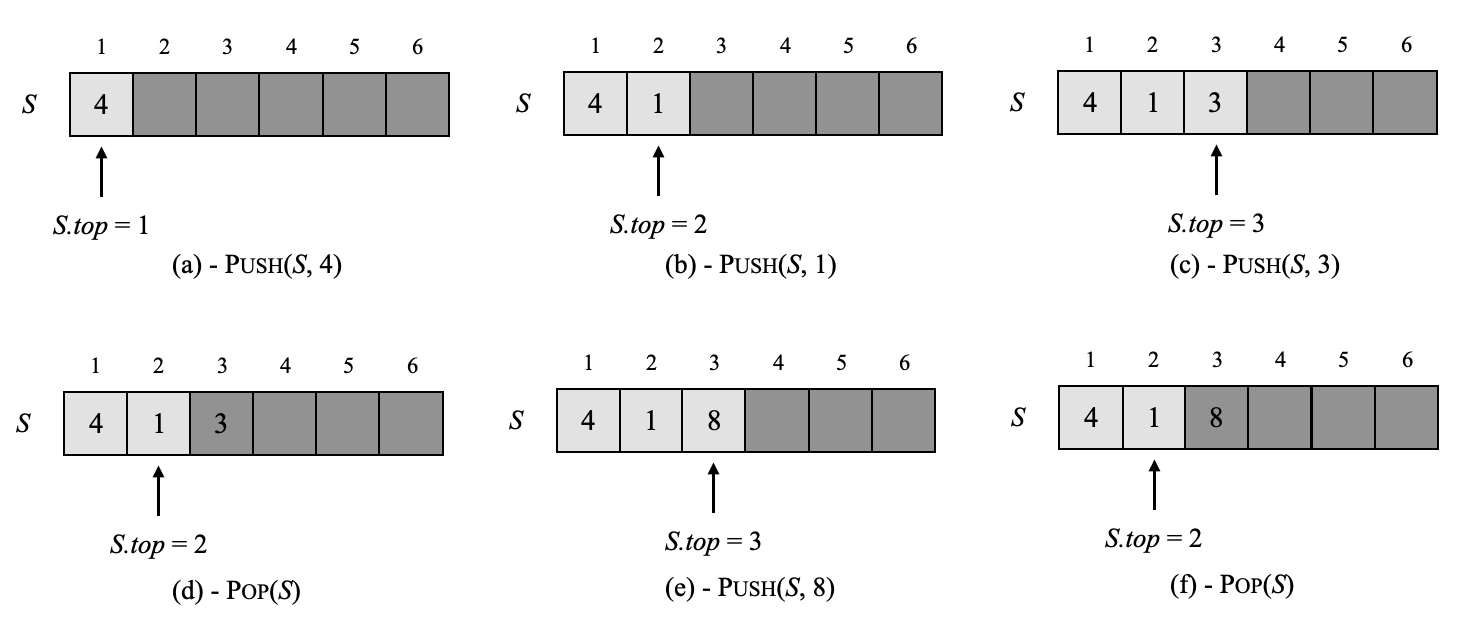
\includegraphics[scale=0.65]{./hw7-8q3.png}


%%% Problem 4 %%%
\newpage
\begin{prob} \textbf{(10 points)} Exercise 10.1-4.
\end{prob}
Rewrite $\textproc{\textsc{Enqueue}}$ and $\textproc{\textsc{Dequeue}}$ to detect underflow and overflow of a queue.

\solution

Because a queue of size $n$ is designed to fit $n-1$ elements, it is full when $Q.\text{head} == Q.\text{tail} + 1$ or when $Q.\text{tail} == Q.\text{length}$ if $Q.\text{head}$ is still pointing to the first position.
\begin{algorithmic}[1]
\Function{Enqueue}{$Q$, $x$}
	\If {$Q.\text{head} == Q.\text{tail} + 1 \textbf{ or } (Q.\text{head} == 1 \textbf{ and } Q.\text{tail} == Q.\text{length})$}
		\State \textbf{error} "overflow" \Comment{throws error and returns}
	\EndIf
	\State $Q[Q.\text{tail}] = x$
        \If {$Q.\text{tail} == Q.\text{length}$}
            	\State $Q.\text{tail} = 1$
        \Else 
        		\State $Q.\text{tail} = Q.\text{tail} + 1$
	\EndIf
\EndFunction
\end{algorithmic}

A queue becomes empty when the head and tail pointer point to the same position.
\begin{algorithmic}[1]
\Function{Dequeue}{$Q$}
	\If {$Q.\text{head} == Q.\text{tail}$}
		\State \textbf{error} "underflow" \Comment{throws error and returns}
	\EndIf
	\State $x = Q[Q.\text{head}]$
        \If {$Q.\text{head} == Q.\text{length}$}
        		\State {Q.\text{head} = 1}
        \Else
        		\State {Q.\text{head} = Q.\text{head} + 1}
	\EndIf
        \State \textbf{return} x
\EndFunction
\end{algorithmic}


%%% Problem 5 %%%
\newpage
\begin{prob} \textbf{(10 points)} Exercise 10.1-6.
\end{prob}
Show how to implement a queue using two stacks. Analyze the running time of the queue operations.

\solution

Let's create two empty stacks $A$ and $B$. The stack $A$ is used to accept elements added to the queue. The stack $B$ is mainly used when we want to remove elements from the queue.

The definition of $\textproc{\textsc{Enqueue}}$ is trivial,

\begin{algorithmic}[1]
\Function{Enqueue}{$A$, $B$, $x$}
	\State $\textproc{\textsc{Push}}(A, x)$ \Comment{call the $\textproc{\textsc{Push}}$ api of stack}
\EndFunction
\end{algorithmic}

We fill $B$ by popping elements from $A$. Thus, $B$ stores what have been in $A$ in reversed order. This allows us to dequeue simply by popping from $B$. We refill $B$ the same way when it becomes empty. The definition of $\textproc{\textsc{Dequeue}}$ is as follows,

\begin{algorithmic}[1]
\Function{Dequeue}{$A$, $B$}
	\If {\textproc{\textsc{Stack-Empty}}(B)}
		\While {\textbf{not} \textproc{\textsc{Stack-Empty}}(A)}
			\State $x = \textproc{\textsc{Pop}}(A)$
			\State $\textproc{\textsc{Push}}(B, x)$
		\EndWhile
	\EndIf
	\State $\textbf{return } \textproc{\textsc{Pop}}(B)$
\EndFunction
\end{algorithmic}

$\textproc{\textsc{Enqueue}}$ runs in $O(1)$-time because $\textproc{\textsc{Push}}$ runs in $O(1)$-time. $\textproc{\textsc{Dequeue}}$ runs in $O(n)$-time in the worst case (i.e. stack $B$ is empty), otherwise it runs in $O(1)$-time by calling $\textproc{\textsc{Pop}}$ on $B$ once.

Note that $\textproc{\textsc{Push}}$, $\textproc{\textsc{Pop}}$, $\textproc{\textsc{Stack-Empty}}$ are stack related functions defined in CLRS on page 233.


%%% Problem 6 EC %%%
\newpage
\begin{prob} \textbf{(Extra Credit)} Exercise 10.1-7.
\end{prob}

%%% Problem 7 %%%
\newpage
\begin{prob} \textbf{(10 points)} Exercise 10.2-2.
\end{prob}
Implement a stack using a singly linked list $L$. The operations $\textproc{\textsc{Push}}$ and $\textproc{\textsc{Pop}}$ should still take $O(1)$-time.

\solution

To achieve "push", we simply link the next pointer of a new node to the current head of a list $L$.

\begin{algorithmic}[1]
\Function{Push}{$L$, $\textit{value}$}
	\State init a new node $x$
	\State $x.\text{key} = \textit{value}$
	\State $x.\text{next} = L.\text{head}$
	\State $L.\text{head} = x$
\EndFunction
\end{algorithmic}


To achieve "pop", we want to remove the element lastly added, which is at the head of the list. 

\begin{algorithmic}[1]
\Function{Pop}{$L$}
	\State $x = L.\text{head}$
	\If {$x \ne \textproc{\textsc{nil}}$}
		\State \textit{key} $= x$.key
		\State $L.\text{head} = L.\text{head}.\text{next}$
		\State \textbf{return} \textit{key}
	\Else
		\State \textbf{error} "underflow"
	\EndIf
\EndFunction
\end{algorithmic}

Pointer manipulations and if condition checks are constant time operations in the above two functions. Thus, their runtimes are $O(1)$.


%%% Problem 8 %%%
\newpage
\begin{prob} \textbf{(10 points)} Exercise 10.2-6.
\end{prob}

The dynamic-set operation \textproc{\textsc{Union}} takes two disjoint sets $S_1$ and $S_2$ as input, and it returns a set $S = S_1 \cup S_2$ consisting of all the elements of $S_1$ and $S
_2$. The sets $S_1$ and $S_2$ are usually destroyed by the operation. Show how to support \textproc{\textsc{Union}} in $O(1)$ time using a suitable list data structure.

\solution

Suppose the data structure we used to store $S_1$ and $S_2$ is a circular, doubly linked list with a sentinel. We are going to do some pointer manipulations to combine the two lists into one. Let's call the two lists $A$ and $B$ and try to link $A$'s sentinel's prev ("tail") to the $B$'s sentinel's next ("head").

\begin{algorithmic}[1]
\Function{Union}{$A$, $B$}
	\State $A$.nil.prev.next $ = B$.nil.next	\Comment{link $A$'s "tail" with $B$'s "head"}
	\State $B$.nil.next.prev $ = A$.nil.prev
	\State $B$.nil.prev.next $ = A$.nil		\Comment{link $A$'s sentinel with $B$'s "tail"}
	\State $A$.nil.prev $ = B$.nil.prev
	\State \textbf{delete} $B$.nil				\Comment{the sentinel of $B$ is no longer needed}
\EndFunction
\end{algorithmic}

The four pointer manipulations and the delete are constant-time operations. We thus manage to do \textproc{\textsc{Union}} in $O(1)$ time.


%%% Problem 9 %%%
\newpage
\begin{prob} \textbf{(10 points)} Exercise 10.4-2.
\end{prob}
Write an $O(n)$ time recursive procedure that, given an $n$-node binary tree, prints out the key of each node in the tree.

\solution

 Suppose we want to do a pre-order traversal of the tree.

\begin{algorithmic}[1]
\Function{PrintTree}{T}
	\If {$T$.root $\ne$ \textproc{\textsc{nil}}}
		\State \textbf{print } $T$.root.key
		\State $\textproc{\textsc{PrintTree}}(T.\text{root.left})$
		\State $\textproc{\textsc{PrintTree}}(T.\text{root.right})$
	\EndIf
\EndFunction
\end{algorithmic}

The print function has the recurrence $T(n) = 2T(n/2) + 1$. Using the master theorem, we have $\log_b^a = \log_2^2 = 1 < 0 = c$. Thus, the runtime is $O(n)$.


%%% Problem 10 EC %%%
\newpage
\begin{prob} \textbf{(Extra Credit)} Problem 10-1.
\end{prob}


%%% Problem 11 %%%
\newpage
\begin{prob} \textbf{(10 points)} Exercise 12.2-5.
\end{prob}
Show that if a node in a binary search tree has two children, then its successor has no left child and its predecessor has no right child.

\solution

If a node has two children, it means that its predecessor and successor are under it. A successor exists in the right subtree, and it is the smallest element of the right subtree. We can find the successor at the end of a path going downward to the left. If it were to have a left child (i.e. a child that is even smaller), it shouldn't have been the minimum value for the right subtree: a contradiction. On the other hand, the predecessor exists in the left subtree, and it is the maximum element of the left subtree. We find the predecessor at the end of a path going downward to the right. If it were to have a right child (i.e. a child that is even greater), it shouldn't have been the maximum value of the left subtree: a contradiction. 


%%% Problem 12 %%%
\newpage
\begin{prob} \textbf{(10 points)} Exercise 12.2-7.
\end{prob}
An alternative method of performing an in-order tree walk of an $n$-node binary search tree finds the minimum element in the tree by calling $\textproc{\textsc{Tree-Minimum}}$ and then making $n - 1$ calls to $\textproc{\textsc{Tree-Successor}}$. Prove that this algorithm runs in $\Theta{(n)}$ time.

\solution

To help analyze the runtime of the algorithm, we keep track of how many times each node is visited while doing these procedures. $\textproc{\textsc{Tree-Minimum}}$ visits nodes along a path downward to the left from the root. Those nodes are visited once. By calling $\textproc{\textsc{Tree-Successor}}$ on the smallest node (let's call it $N_1$), we find the successor to be its direct parent node $N_2$, which have been visited twice. Now, we aim to find the successor of $N_2$. We will either going upward when $N_2$ does not have a right child, or going downward when it does. If we decide to move upward, we will no longer visit nodes below $N_2$. If we go downward, we eventually will visit back to $N_2$ and up in order to find the successor of the largest value of $N_2$'s right subtree. Regardless which direction we are going, we won't visit a node more than thrice.

The algorithm is upper bounded by $O(3n) = O(n)$ time. It is lower bounded by $\Omega{(n)}$ because there are $n$ nodes in the tree to be visited at least once. Overall, the algorithm runs in $\Theta{(n)}$ time.


%%% Problem 13 %%%
\newpage
\begin{prob} \textbf{(10 points)} Exercise 12.3-3
\end{prob}
We can sort a given set of $n$ numbers by first building a binary search tree containing these numbers (using $\textproc{\textsc{Tree-Insert}}$ repeatedly to insert the numbers one by one) and then printing the numbers by an in-order tree walk. What are the worst-case and best-case running times for this sorting algorithm?

\solution

In the worst case, the numbers are already sorted when they are inserted. The BST will be extremely unbalanced. $\textproc{\textsc{Tree-Insert}}$ has to visit $n-1$ nodes in order to insert the last number into the right spot. It has to visit $n-2$ nodes to insert the second to last number. So on so forth, the cost is $(n-1) + (n-2) + (n-3) + ... + 2 + 1 = ((1 + n - 1)n)/2 = \Theta{(n^2)}$, which is the worst-case runtime.

In the best case, numbers are arranged in a way such that $\textproc{\textsc{Tree-Insert}}$ gradually forms a balanced BST while inserting the numbers one by one. We know that a balanced binary tree of $n$ nodes have height $\Theta{(\lg n)}$. The algorithm is clearly upper bounded by $O(n \lg n)$ because at most the last number to be inserted visits $\lg n$ nodes (the height of the tree) to find its spot. We have shown that any comparison-based sorting algorithm is lower bounded by $\Omega{(n \lg n)}$. Thus, the runtime of this algorithm is $\Theta{(n \lg n)}$.


%%% Problem 14 EC %%%
\newpage
\begin{prob} \textbf{(Extra Credit)} Problem 12-3.
\end{prob}

%%% Problem 15 EC %%%
\begin{prob} \textbf{(Extra Credit)} Problem 10-2.
\end{prob}

%%% Problem 16 EC %%%
\begin{prob} \textbf{(Extra Credit)} Problem 15-6.
\end{prob}

%%% Problem 17 %%%
\newpage
\begin{prob} \textbf{(50 points)}
\end{prob}

\noindent Implement a hash for text.  Given a string as input,  construct a hash with words as keys, and word counts as values.  Your implementation should include:

\begin{itemize}
\item a hash function that has good properties for text

\item storage and collision management using linked lists

\item operations:  insert(key,value), delete(key), increase(key), find(key), list-all-keys
\end{itemize}

\noindent Output the list of words together with their counts on an output file.  For this problem,you  cannot  use  built-in-language  datastuctures  that  can  index  by  strings  (like  hashtables).  Use a language that easily implements linked lists, like C/C++.

\noindent You can test your code on “Alice in Wonderland” by Lewis Carroll, at \href{http://www.ccs.neu.edu/home/vip/teach/Algorithms/7_hash_RBtree_simpleDS/hw_hash_RBtree/alice_in_wonderland.txt}{link}

\noindent The test file used by TA will probably be shorter.
\\

\noindent (Extra Credit) Find a way to record not only word counts, but also the positions in text.  For each word, besides the count value, build a linked list with positions in the given text.  Output this list together with the count.

\solution

Please refer to code listed on the next page.


%%% Problem 18 %%%
\newpage
\begin{prob} \textbf{(50 points)}
\end{prob}

\noindent Implement  a  red-black  tree,  including  binary-search-tree  operations \textit{sort, search, min, max, successor, predecessor} and  specific  red-black  procedures \textit{rotation, insert, delete.}  The delete implementation is Extra Credit (but highly recommended).
\\

\noindent Your code should take the input array of numbers from a file and build a red-black tree with this input by sequence of “inserts”.  Then interactively ask the user for an operational command like “insert x” or “sort” or “search x” etc, on each of which your code rearranges the tree and if needed produces an output.  After each operation also print out the height of the tree.
\\

\noindent You  can  use  any  mechanism  to  implement  the  tree,  for  example  with  pointers  and struct objects in C++, or with arrays of indices that represent links between parent and children.  You cannot use any tree built-in structure in any language.

\solution

Please refer to code listed on the next page.

\end{document}